\section{Border Gateway Protocol}

\subsection{Overview}

\paragraph{BGP} An exterior gateway protocol designed to exchange routing and reachability information among autonomous systems (AS) on the Internet (update messages over TCP). Routing decisions are made based on paths (list of ASes) and network policies / rule-sets configured by a network admin. For routing within an AS, see the Interior BGP (iBGP). %TODO: slides 43-55 for details

\paragraph{Path-Vector Routing Protocol} A routing protocol that maintains the received path information and updates it dynamically. Each entry of a routing table contains the destination network, the next router and the path to reach the destination.

In BGP, border routers (eBGP peers) send path-vector messages (over TCP) to advertise the reachability of networks. Each router verifies the received advertisements according to its policy.


\subsection{Security of BGP}

\paragraph{BGP Hijacking} BGP routers accept advertised routes from other BGP routers by default (automatic and decentralized routing). This allows for accidental or malicious disruption (blackhole, redirection, interception) by taking over an entire IP prefix(es) ($\approx$ AS) and illegitimately advertise for it. A stronger variation is to originate a more specific (longer) prefix fitting the victim's address space. Traffic will follow the longest matching prefix. Either set up an AS and border router or compromise an already existing router.

Correcting this vulnerability (e.g. crypto keys to verify identity of routers) is technically and economically challenging due to the extend BGP is embedded in the core of the Internet.

\textbf{Problem 1:} BGP does not validate the origin of advertisements.

\textbf{Problem 2:} BGP does not validate the content of advertisements. An AS can easily modify a BGP path (remove an AS to make path look shorter or to attract sources avoiding that specific AS; add an AS to trigger loop detection = DoS or make it look like it has better connections).

\paragraph{BGP Interception}
Hijacked traffic is captured but still reaches the original / legitimate destination.

\textbf{BGP poisoning:} the hijacked prefix is only announced to and used by some neighbors by triggering loop detection s.t. specific ASes don't accept certain announcements. %TODO: better

\textbf{BGP communities:} can be used to make sure announcements only reach certain ASes, no involuntary learning by peers. Possible by using the \textit{NoExportSelect} action for a specific AS.

\paragraph{Dangers of BGP Hijacking}
\begin{itemize}
    \item Interception / redirection of non-encrypted data (DNS, HTTP, etc.)
    \item Deriving timing information of encrypted data (fingerprinting).
    \item Dropped packages (blackholes) and widespread outages.
    \item Very hard to notice, needs cooperation of ISPs.
    \item Obtaining fake (TLS) certificates.
    \item Deanonymizing TOR users.
    \item Hijacking DNS requests.
    \item Partition the Bitcoin network.
    \item etc.
\end{itemize}

\paragraph{Other Attacks on BGP}
Most of these attacks are easy to defend against and no longer a big concern. %TODO: how?

\begin{itemize}
    \item Performing a DoS attach by overloading the link between BGP routers which causes packet loss / delay or sending bogus TCP packets that falsely close a session (FIN/RST) or flood a router (SYN).
    \item Eavesdropping or tampering with messages by tapping the link. %TODO: ?
\end{itemize}

\subsection{Countermeasures}

\paragraph{Desired Properties}
We only want ASes that actually own an IP prefix to be allowed to announce it (cryptographic authentication) and routing messages need to be authenticated by all ASes on the path (cryptographic protection, no modification of announcements).

\paragraph{Best Current Practices}
They are not good enough since they don't address the fundamental problems (who owns an IP address block, is the AS path valid, do data packets actually follow chosen route, etc.)\footnote{See MANRS (Mutually Agreed Norms for Routing Security) for current security efforts.}

\begin{itemize}
    \item Securing the BGP peering session between routers (authentication and priority over other traffic). %TODO: how?
    \item Filtering routes by prefix and AS path.
    \item Filters to block unexpected control traffic.
    \item Filtering based on entries in the Internet Routing Registries (IRRs) which contains prefixes.
\end{itemize}

\paragraph{Solution 1: Origin Authentication}
Enable issuance of Route Origination Authorizations (ROAs) with a Resource Public-Key Infrastructure (RPKI). They state which AS is authorized to announce certain IP prefixes and determine the maximum length of such.

\textbf{RPKI:} prove ownership of resources by creating a secure database that maps Internet number resources to a trust anchor (e.g. regional Internet registries - RIRs) and utilizing certificates that prove that an AS holds a specific resource. Certificates follow the same delegation as IP addresses from RIRs and are signed / distributed / verified out-of-band (does not require a modification to BGP).

\begin{figure}[h]
	\centering
	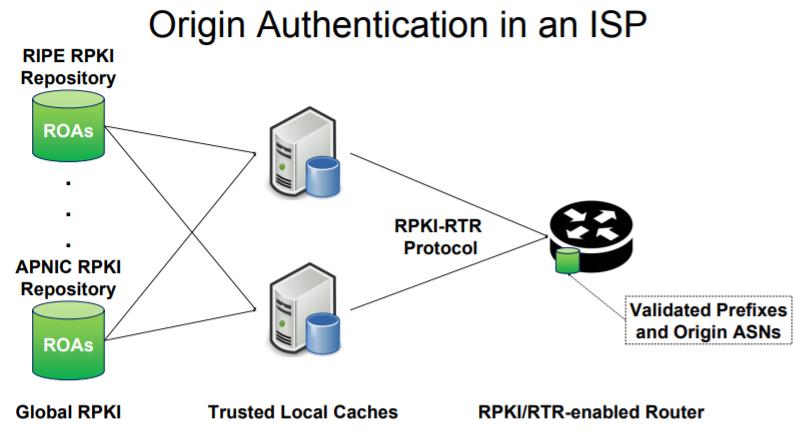
\includegraphics[scale=0.5]{images/8-origin.PNG}
	\caption{Origin authentication in an ISP.}
	\label{fig:bgp1}
\end{figure}

\textbf{Operation:} 1) Receive announcement for prefix v from AS M. 2) Check against ROAs in RPKI for prefix v. 3) Accept if valid ROA for AS M is found, else drop announcement.

\textbf{Not enough:} A malicious AS can append itself on the path with a valid ROA for certain prefix and attract (a fraction of) traffic for legitimate AS.

\paragraph{Solution 2: BGPsec}
BGPsec secures the AS-PATH attribute in BGP announcements and prevents the crafting of a valid origin by prepending ASes along with path poisoning. It's basically origin authentication $+$ cryptographic signatures. Received messages are signed to prove that a path was correctly updated (next AS is included in the signature). %TODO: more

BGPsec can validate that the AS path indicates the actual order of traversed ASes and disables modifications (adding/removing an AS). RPKI is used to verify AS key material (similar to solution 1).

BGPsec is in incremental deployment which allows for protocol downgrade attacks (if security is not prioritized when dealing with non-BGPsec BGP routers). It is challenging to figure out how to effectively prioritize security (over business relationships). Furthermore, performance is degraded since BGPsec does not allow for prefix aggregation and involves complex crypto (slower convergence).

Challenges for large-scale deployment include: different message formats, complete and accurate registries and PKI. In general, upgrading equipment is expensive, cooperation amongst many entities is required and the benefits are unclear for first-movers.

\paragraph{Extensive Monitoring}
Another approach to problem 2. BGP update messages are monitored and compared to past history. Remember which AS originates which prefix and AS-level edges / paths. Delay adoption of unfamiliar routes if possible.

This can be realised with an out-of-band detection mechanism (e.g. \textit{ARTEMIS}, \textit{Prefix Hijack Alert System}, etc.).

\paragraph{SCION}
Proposal to redesign inter-domain routing since BGP was not created with security in mind. Introduces trusted entities, enables simple security patches, etc. Other approaches include Named-Data Networking / Information-Centric Networking, Accountable Internet Protocol, Passport: Secure and Adoptable Source Authentication, etc.
